\documentclass{article}
\usepackage{graphicx}
\usepackage{xcolor}
\graphicspath{ {./images/} }
\usepackage[utf8]{inputenc}
\usepackage{hyperref}
\usepackage{xcolor}
\usepackage{listings}

\definecolor{mGreen}{rgb}{0,0.6,0}
\definecolor{mGray}{rgb}{0.5,0.5,0.5}
\definecolor{mPurple}{rgb}{0.58,0,0.82}
\definecolor{backgroundColour}{rgb}{0.95,0.95,0.92}

\lstdefinestyle{CStyle}{
    backgroundcolor=\color{backgroundColour},   
    commentstyle=\color{mGreen},
    keywordstyle=\color{magenta},
    numberstyle=\tiny\color{mGray},
    stringstyle=\color{mPurple},
    basicstyle=\footnotesize,
    breakatwhitespace=false,         
    breaklines=true,                 
    captionpos=b,                    
    keepspaces=true,                 
    numbers=left,                    
    numbersep=5pt,                  
    showspaces=false,                
    showstringspaces=false,
    showtabs=false,                  
    tabsize=2,
    language=C
}

\title{Rapport de Projet en Algorithimique et Structure de Données 2}
\author{Nourry Celian & Numéro Étudiant : 22002895}
\date{Date de rendu : le 21/04/2024}

\begin{document}

\maketitle
\section*{Étape 1}
Alphabet : CROY\newline
Motif 1 : CO*Y+OR\newline
Motif 2 : C+OY+O?Y*R+\newline\newline
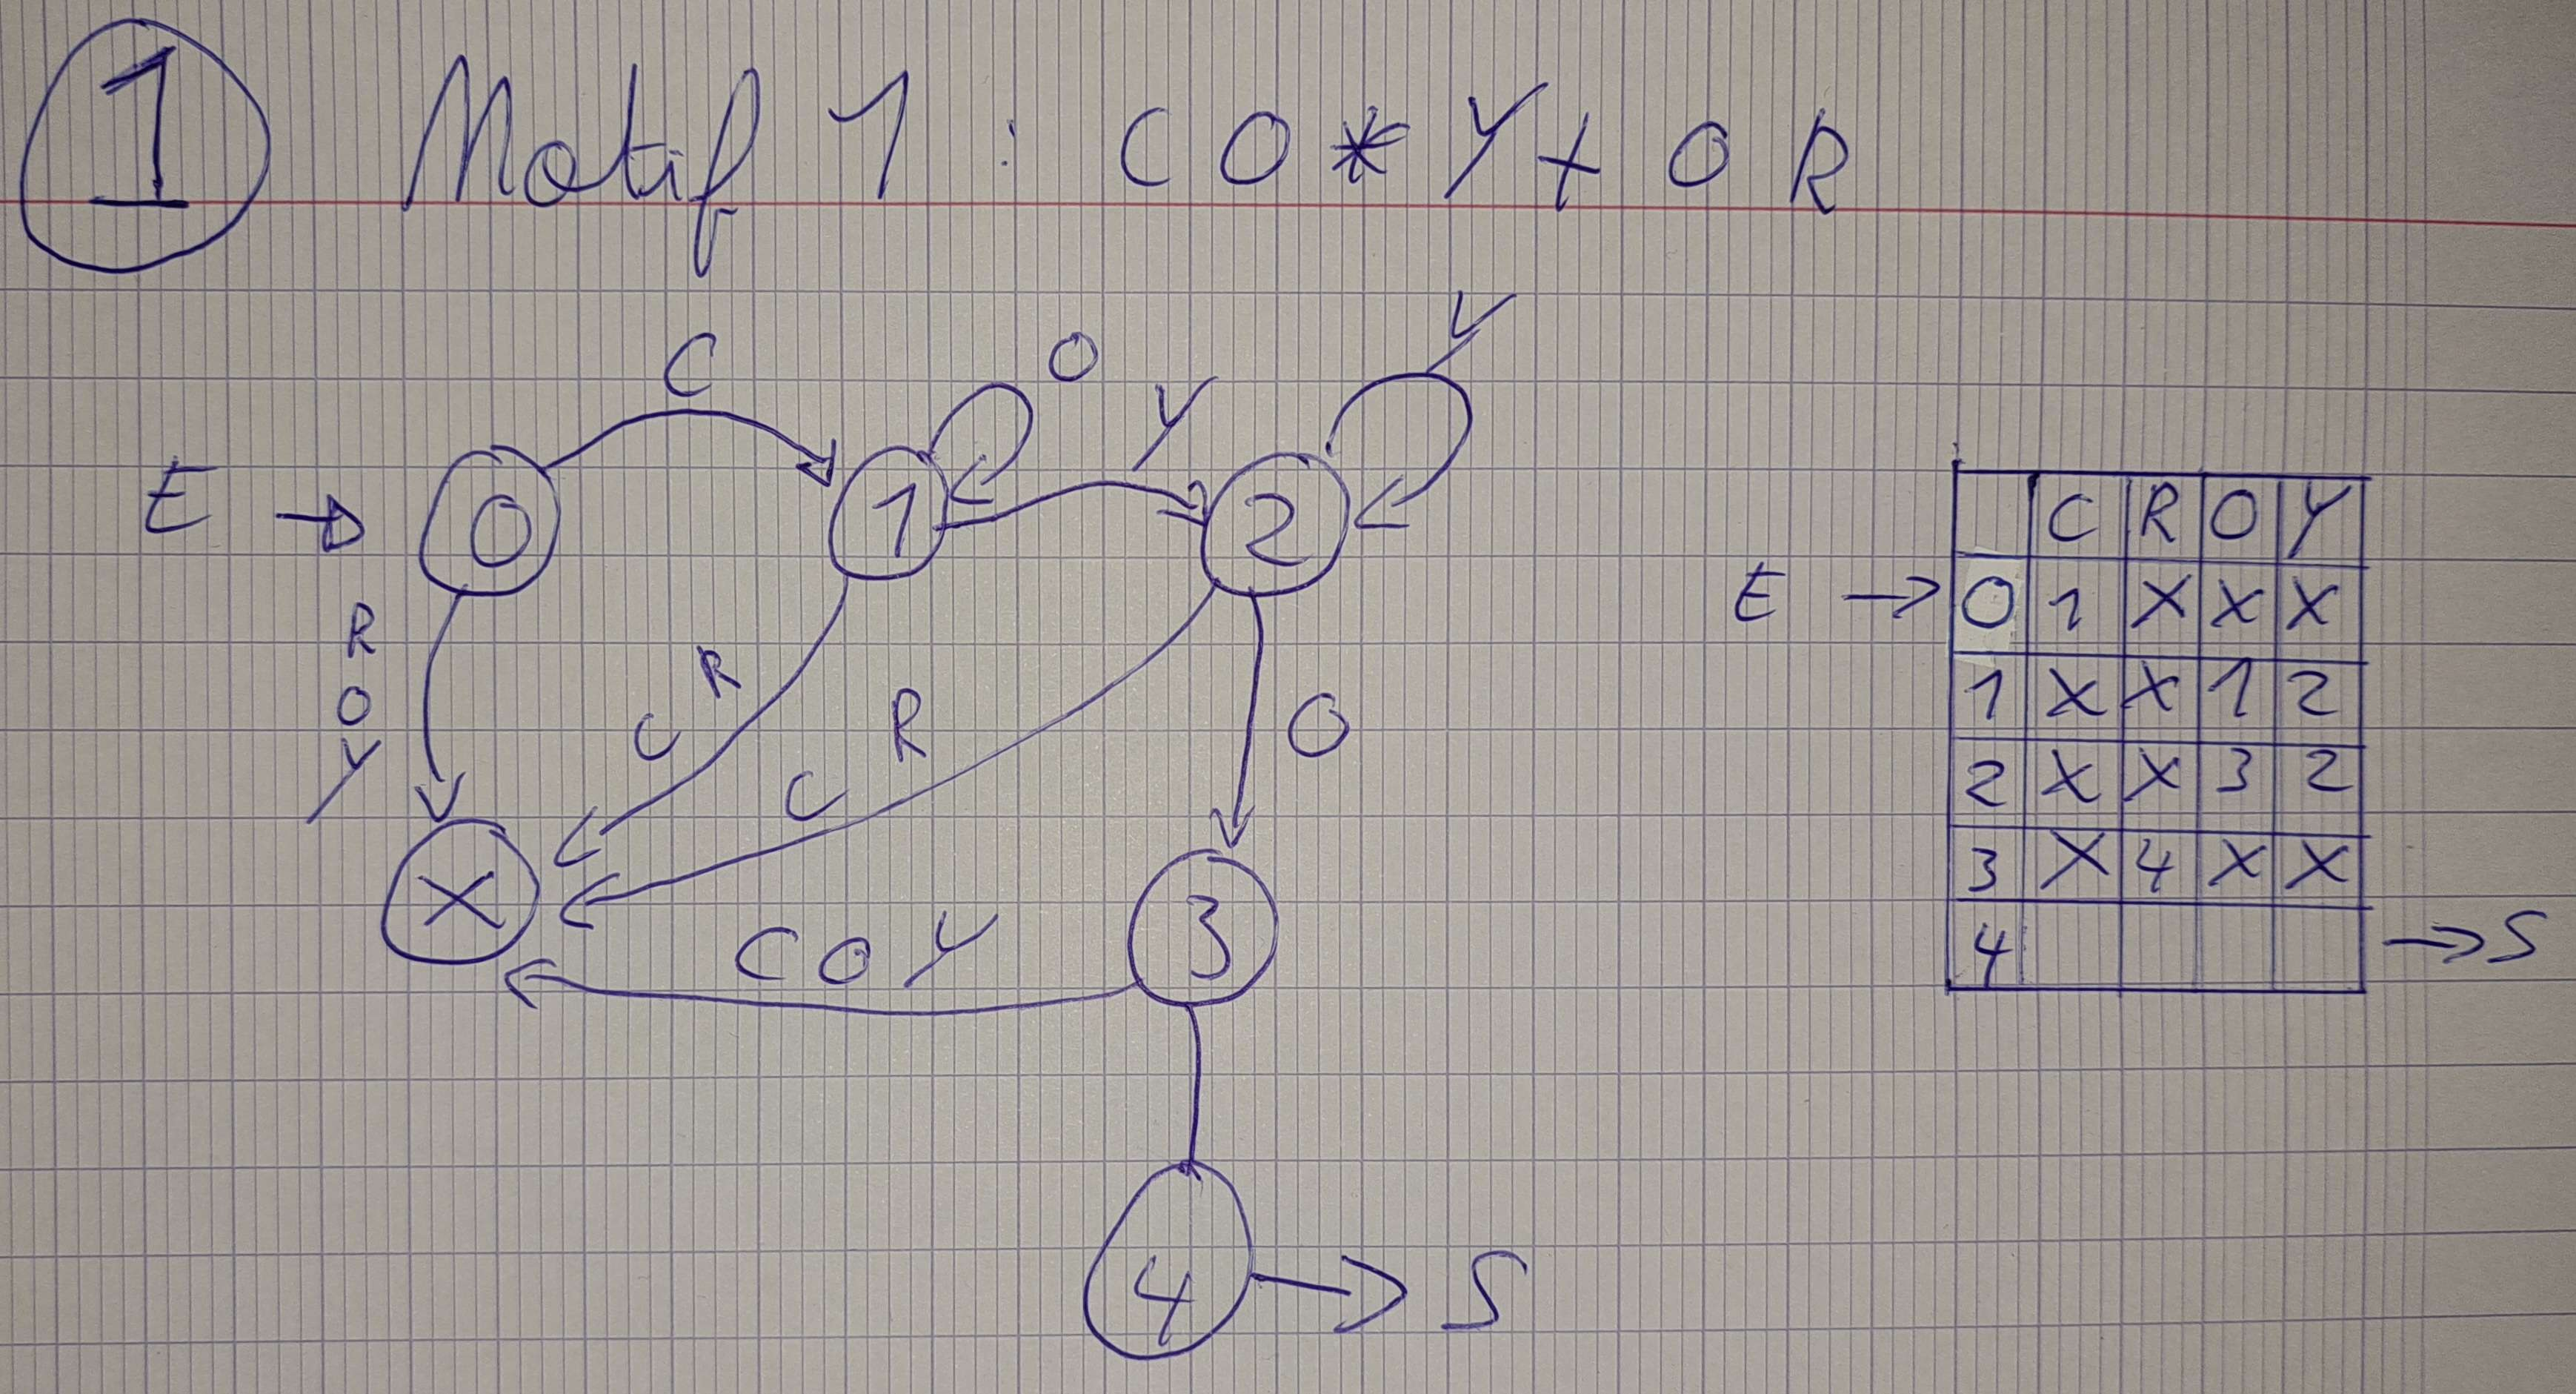
\includegraphics[scale=0.1]{images/Motif 1.jpg}
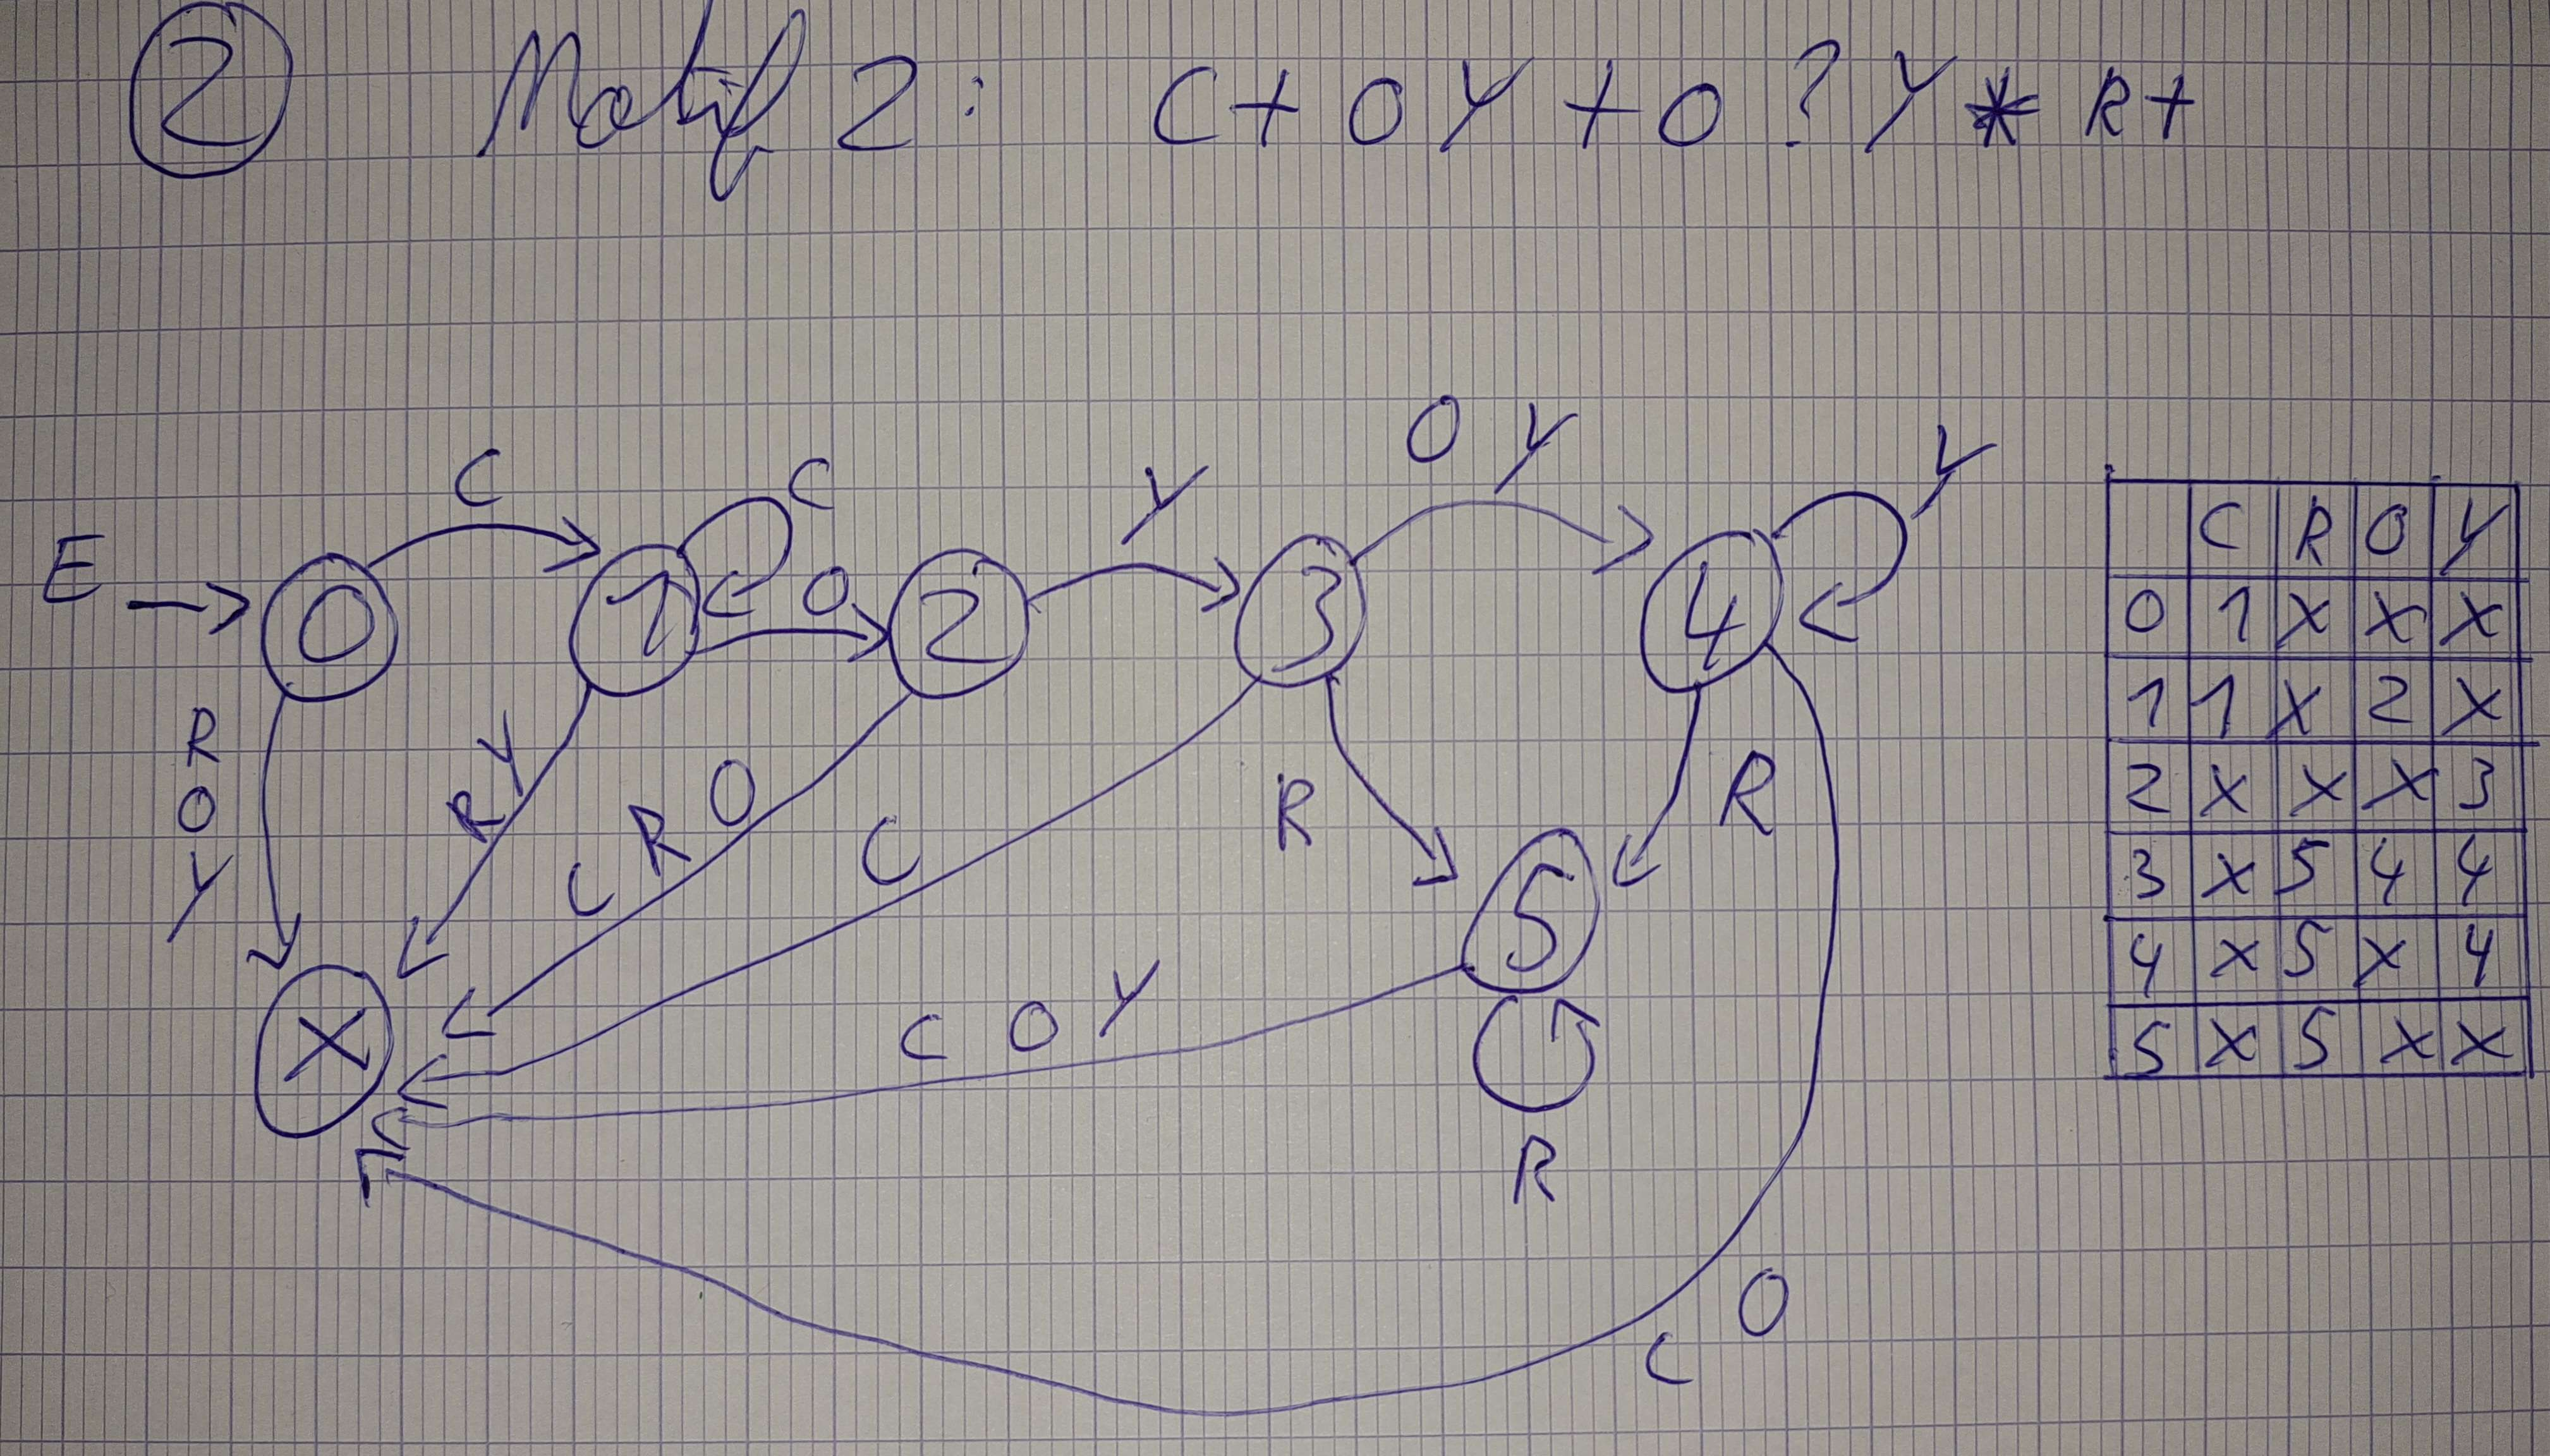
\includegraphics[scale=0.1]{images/Motif 2.jpg}
\section*{Étape 2}

Dans le code ci-dessous, on va d'abord définir des valeurs constantes, dont "TAB SIZE" qui est de 4000 et qui sera la taille de notre tableau de lettres. On va aussi définir "ALPHABET SIZE" qui sera la taille de notre alphabet. On créer la première structure de données "INFO MOTS". Cette structure de données est la plus importante du projet puisque c'est elle qui va nous servir à stocker les différentes informations demandées au cours des étapes.\newline\newline
La structure "INFO MOTS" continent :

    - les lettres du mot en question dans la chaîne de caractères "mot[TAB SIZE]"\newline
    - la position du début et de fin du mot dans la chaîne de 2 entiers "position[2]", où "position[0]" est l'indice du début du mot et "position[1]" est l'indice de la fin du mot\newline
    - le nombre d'occurrences de ce mot dans le TABLEAU (pour l'étape 5) dans la variable "doublons"\newline
    - le nombre de points que ce mot rapporte en tout dans la variable "points" \newline
    - un booléen "prem lu" utilisé à l'étape 5 savoir si ce mot est lu pour la première fois dans le tableau ou non\newline\newline
On créer également la structure "ALPHABET", qui contient une chaîne de caractère qui représente les lettres de notre alphabet, ainsi qu'une chaîne d'entiers qui représente combien de points vaut chacune des lettres de notre alphabet.\newline
\begin{lstlisting}[style=Cstyle]
#define TAB_SIZE 4000
#define ALPHABET_SIZE 4

typedef struct INFO_MOTS{
    char mot[TAB_SIZE];
    int position[2];
    int doublons;
    int points;
    bool prem_lu;
} INFO_MOTS;

typedef struct ALPHABET {
  char lettres[ALPHABET_SIZE];
  int points[ALPHABET_SIZE];
} ALPHABET;
\end{lstlisting}
Ces informations seront utiles dans le traitement du tableau que nous créons dans le code ci-dessous avec notre ALPHABET personnalisé. Nous initialisons d'abord notre tableau de 4000 caractères, puis notre alphabet avec nos lettres 'C', 'R', 'O' et 'Y' avec leurs points respectifs 8, 20, 4 et 6. La fonction "creation-tableau()" va simplement choisir un nombre entre 0 et ALPHABET-SIZE (4) qui sera l'indice mit dans l'attribut "lettres" de notre alphabet. Cela a pour effet de choisir une lettre aléatoire de notre alphabet que nous allons mettre dans notre TABLEAU. Nous allons faire cela jusqu'à que la TABLEAU soit remplis grâce à une boucle for sur TAB-SIZE (4000 boucles).\newline

\begin{lstlisting}[style=Cstyle]
//Initialisation du tableau de 4000 caracteres
char TABLEAU[TAB_SIZE];
ALPHABET alphabet;

/* Algorithme pour generer le TABLEAU aleatoire ci-dessous*/
void creation_TABLEAU(void){
  alphabet.lettres[0] = 'C'; alphabet.lettres[1] = 'R'; alphabet.lettres[2] = 'O'; alphabet.lettres[3] = 'Y';
  alphabet.points[0] = 8; alphabet.points[1] = 20; alphabet.points[2] = 4; alphabet.points[3] = 6;

  srand(time(NULL));
  int random_int;

  for (int i = 0, a = 0; i < TAB_SIZE; i++, a++){
    random_int = rand() % ALPHABET_SIZE;
    TABLEAU[i] = alphabet.lettres[random_int];
  }
}
\end{lstlisting}

Pour commencer l'analyse des informations du TABLEAU, nous allons créer une fonctions utilisant les automates pour pouvoir gérer les expressions régulières de nos deux motifs. Les fonctions "automate" et "get-type" ont été reprises des codes fournis par F. Balmas en cours.\newline

\begin{lstlisting}[style=Cstyle]
#define ETATENTREE 0
#define ETATERREUR -1
#define NBTYPES 5

#define MOTIF_1

enum types {C, R, O, Y, AUTRE};

#ifdef MOTIF_1
#define ETATSORTIE 10
#define NBETATS 4
int ttransit[NBETATS][NBTYPES] = {{ 1, -1, -1, -1, -1 },
                                  { -1, -1, 1, 2, -1 },
                                  { -1, -1, 3, 2, -1 },
                                  { -1, 10, -1, -1, -1 }};
#endif

#ifdef MOTIF_2
#define ETATSORTIE 5
#define NBETATS 6
int ttransit[NBETATS][NBTYPES] = {{ 1, -1, -1, -1, -1 },
                                  { 1, -1, 2, -1, -1 },
                                  { -1, -1, -1, 3, -1 },
                                  { -1, 5, 4, 4, -1 },
                                  { -1, 5, -1, 4, -1 },
                                  { -1, 5, -1, -1, -1 }};
#endif

enum types get_type(char str) {
    switch (str) {
        case 'C': return C;
        case 'R': return R;
        case 'O': return O;
        case 'Y': return Y;
        default: return AUTRE;
    }
}

char automate(char *str, char etat, int *len) {
    for (int i = 0; str[i] != '\0'; i++) {
        enum types t = get_type(str[i]);
        etat = ttransit[(int)etat][t];

        //La taille du mot incremente tant que les caracteres lus ne sont pas une erreur
        (etat == ETATERREUR) ? *len = 0 : (*len)++;

        #ifdef MOTIF_1
        if(etat == ETATERREUR || etat == ETATSORTIE) return etat;
        #endif

        #ifdef MOTIF_2
        if(etat == ETATERREUR) return etat;
        if (etat == ETATSORTIE && ttransit[(int)etat][get_type(str[i + 1])] == ETATERREUR) return etat; //Verification pour R+, on s'arrete pas de lire tant qu'il n'y a pas d'erreur (donc pas de R)
        #endif
    }
    return etat;
}
\end{lstlisting}
\newline
Notre automate prends une chaîne de caractère en paramètre qui va être analysée grâce aux chaînes d'entiers "ttransit" qui respectent les expressions régulières de nos deux motifs. Notre état d'entrée est toujours 0 et celui d'erreur est toujours -1. L'automate fait une boucle sur chacun des caractères de la chaîne de caractères pris en paramètres. L'état est modifié dans la boucle à chaque lettre que l'automate est en entrain d'analyser grâce à la fonction get-type() qui renvoie la lettre correspondante à str[i]. Chaque ligne représente une lettre, qui sont C, R, O, Y ou AUTRE respectivement. Pour le MOTIF 1, l'automate s'arrête dès qu'il renvoie un état d'erreur ou un état de sortie (10). Cependant, le MOTIF 2 est plus spécial puisqu'il comprendre plusieurs R à la fin de sa chaîne de caractère. Donc si notre automate est dans un état de sortie, il ne va pas directement valider l'expression régulière et va continuer à enregistrer les R jusqu'à tant que l'état suivant est un état d'erreur. L'état de sortie est également mit à 5 pour pouvoir manipuler celui-ci comme un état normal. Il y a également un pointeur d'entier prit en paramètre ("len") qui est utilisé pour mesurer la taille d'une chaîne de caractère valide. La valeur de cette variable augmente tant que l'automate ne tombe pas sur un état d'erreur, sinon la variable est réinitialisée à 0.\newline\newline
L'analyse du tableau se fait dans la fonction analyse-tableau() qui prend en paramètre une chaîne de caractère (notre tableau de 4000 caractères dans notre cas) et liste d'INFO-MOT "LISTE-MOTS" (qui est vide pour le moment). Le but de cette fonction est de remplir notre structure de donnée "LISTE-MOTS" pour avoir toutes les informations dont nous avons besoins.\newline
\begin{lstlisting}[style=Cstyle]
int analyse_tableau(char *str, INFO_MOTS *LISTE_MOTS){
int occurrences = 0, len = 0;
char *current_ptr = str;

    for (int i = 0; *current_ptr != '\0'; i++, current_ptr++) {
        if (automate(current_ptr, ETATENTREE, &len) == ETATSORTIE) {
            LISTE_MOTS[occurrences].position[0] = i;
            LISTE_MOTS[occurrences].position[1] = i + len;

            char *mot = (char *) malloc((len + 1) * sizeof(char)); if (mot == NULL) { printf("Erreur d'allocation de memoire.\n"); return -1; }

            for (unsigned short int j = i; j < (i + len); j++){
                enum types t = get_type(str[j]);

                switch (t) {
                    case C: LISTE_MOTS[occurrences].points += alphabet.points[0]; break;
                    case R: LISTE_MOTS[occurrences].points += alphabet.points[1]; break;
                    case O: LISTE_MOTS[occurrences].points += alphabet.points[2]; break;
                    case Y: LISTE_MOTS[occurrences].points += alphabet.points[3]; break;
                    default: return -1;
                }
                mot[j - i] = str[j];
            }

            mot[len] = '\0';
            strcpy(LISTE_MOTS[occurrences].mot, mot);
            free(mot);
            occurrences++;
        }
        len = 0;
    }
    return occurrences;
}
\end{lstlisting}
La fonction initialise un entier "occurrences" un 0 qui sera renvoyé à la fin de la fonction et qui sera le nombre total de mots trouvés grâce à l'expression régulière du motif. Pour analyser la totalité de notre tableau, une boucle for est effectuée sur le pointeur du TABLEAU. À chaque boucle, le début du pointeur du tableau avance d'un indice, ce qui fait que la tableau analysé par l'automate se raccourcis à mesure que la boucle for s'effectue. Cela a pour effet d'analyser tout le TABLEAU. Ainsi, à chaque fois que la boucle for tombe sur un mot valide (atterrissant sur un état de sortie avec la fonction automate), la position du mot est enregistré dans notre liste "LISTE-MOTS". On alloue de la mémoire pour une chaîne de caractère sur la taille du mot (avec "len", étant la taille du mot) et on copie celui-ci dans l'attribut mot de notre "LISTE-MOTS". L'attribut point de LISTE-MOTS est également augmenté pour chaque lettre rencontrée.

\section*{Étape 3}
L'étape 3 utilise le même procédé que l'étape 2, il suffit de modifier le define MOTIF-1 en define MOTIF-2 pour que le motif 2 soit prit en compte dans toutes les fonctions précédentes et suivantes.

\section*{Étape 4}
Pour vérifier si les informations que nous récupérons grâce à ces algorithmes sont corrects, nous créons deux chaînes de caractères constantes dont nous connaissons déjà les informations à l'avance.

\begin{lstlisting}[style=Cstyle]
char MOTIF_1_TEST[TAB_TEST_MOTIF_1];
char MOTIF_2_TEST[TAB_TEST_MOTIF_2];
char MOTIF_1_TEST[TAB_TEST_MOTIF_1] = {'C', 'C', 'Y', 'O', 'R', 'C', 'O', 'O', 'O', 'Y', 'O', 'R', 'Y'};
char MOTIF_2_TEST[TAB_TEST_MOTIF_2] = {'C', 'C', 'Y', 'C', 'O', 'Y', 'O', 'R', 'R', 'R', 'O', 'R', 'Y'};
\end{lstlisting}
Dans la chaîne de caractère "MOTIF-1-TEST" initialisée dans le code ci-dessus, nous savons qu'elle a deux occurrence du motif 1, qu'elles sont à l'indice 1 et 6 du tableau et qui valent 38 et 50 points.\newline
Dans la chaîne de caractère "MOTIF-2-TEST", nous savons qu'elle a une occurrence du motif 2, qu'elle est à l'indice 3 du tableau et qui vaut 82 points.\newline\newline
Maintenant, nous pouvons utiliser ces informations connus dans la fonction assert() qui renvoie une erreur si la valeur mit en paramètre n'est pas égale à ce qu'il y après le "=". Nous créons donc une fonction qui fait cela ci-dessous :\newline

\begin{lstlisting}[style=Cstyle]
void assert_verification(INFO_MOTS *LISTE_MOTS_TEMP){

    #ifdef MOTIF_1
    int occurrences = analyse_tableau(MOTIF_1_TEST, LISTE_MOTS_TEMP);
    assert(occurrences == 2);
    assert(LISTE_MOTS_TEMP[0].position[0] == 1);
    assert(LISTE_MOTS_TEMP[1].position[0] == 5);
    assert(LISTE_MOTS_TEMP[0].points == 38);
    assert(LISTE_MOTS_TEMP[1].points == 50);
    #endif

    #ifdef MOTIF_2
    int occurrences = analyse_tableau(MOTIF_2_TEST, LISTE_MOTS_TEMP);
    assert(occurrences == 1);
    assert(LISTE_MOTS_TEMP[0].position[0] == 3);
    assert(LISTE_MOTS_TEMP[0].points == 82);
    #endif
}

int main(void){
    INFO_MOTS *MOTS_MOTIF_1 = (INFO_MOTS *)malloc((TAB_SIZE) * sizeof(INFO_MOTS));
    INFO_MOTS *MOTS_MOTIF_2 = (INFO_MOTS *)malloc((TAB_SIZE) * sizeof(INFO_MOTS));
    assert_verification(MOTS_MOTIF_1);
    assert_verification(MOTS_MOTIF_2);

    free(MOTS_MOTIF_1);
    free(MOTS_MOTIF_2);
}
\end{lstlisting}
\section*{Étape 5}
La fonction pour trouver les doublons avec le hashcode prend en paramètre une chaîne structure de données INFO-MOTS en paramètre qui a été créée grâce à la fonction analyse-tableau() de l'étape 2. Nous utilisons les fonctions de table de hashage et free-liste fournies en cours par F. Balmas. Ces fonctions ont été inchangées.\newline
\begin{lstlisting}[style=Cstyle]
int doublons_hashage(INFO_MOTS *LISTE_MOTS){
int nb_mot_unique = 0, nb_mot = 0;

    init_freeliste();
    init_tabhash();

    while (LISTE_MOTS[nb_mot].mot[0] != '\0'){
        if (search_nom(LISTE_MOTS[nb_mot].mot) == NULL) {
            add_nom(LISTE_MOTS[nb_mot].mot);
            LISTE_MOTS[nb_mot].doublons++;
            LISTE_MOTS[nb_mot].prem_lu = true;
            nb_mot_unique++;
        }
        else for (int i = 0; LISTE_MOTS[i].mot[0] != '\0'; i++ ) if (strcmp(LISTE_MOTS[i].mot, LISTE_MOTS[nb_mot].mot) == 0) LISTE_MOTS[i].doublons++;
        nb_mot++;
    }
    return nb_mot_unique;
}
\end{lstlisting}
La fonction ci-dessus va initialiser un table de hashage et parcourir la liste des mots enregistrés dans la structure de données INFO-MOTS. Grâce à la fonction search-nom(), on peut vérifier si un mot à déjà été rencontré dans la table de hashage. Si le mot n'est pas dans la table de hashage, il y est ajouté avec la fonction add-nom, l'attribut doublons de la structure INFO-MOTS LISTE-MOTS incrémente et on va marquer ce mot comme "premier lu". Si ce mot est déjà dans la table de hashage, on incrémente l'attribut des doublons de tous les mots étant les mêmes dans la liste LISTE-MOTS. Ainsi, il n'y a qu'un seul des doublons de chaque mot qui est marqué comme "premier lu", et tous les mots incrémentent leur attribut "doublons" si un mot est déjà dans la table de hashage. Nous pouvons donc afficher seulement les mots de la LISTE-MOT ayant l'attribue "prem lu" en true, et afficher les doublons.

\section*{Étape 6}
La fonction de triage croissant des mots selon leur nombre de doublons prend en paramètre une structure de donnée INFO-MOTS LISTE-MOTS modifiée par la fonction doublons-hashage() et le nombre d'occurrences totale des mots dans la LISTE-MOTS.\newline
\begin{lstlisting}[style=Cstyle]
void ordre_croissant(INFO_MOTS *LISTE_MOTS, int nb_occ){
    for (int i = 0; i < nb_occ; i++)
        for (int j = 0; j < nb_occ; j++)
            if (LISTE_MOTS[i].doublons > LISTE_MOTS[j].doublons){
                INFO_MOTS temp;
                temp = LISTE_MOTS[i];
                LISTE_MOTS[i] = LISTE_MOTS[j];
                LISTE_MOTS[j] = temp;
            }
}
\end{lstlisting}
La fonction trie naïvement la LISTE-MOT avec leur attribut doublons, comparent chaque doublons i avec chaque doublons j dans deux boucle for. Si l'attribut doublons i de LISTE-MOT est plus grand que l'attribut doublons j de LISTE-MOT, les deux sont inter changés. Cela a pour effet de trier la liste, malgré son inefficacité.

\section*{Étape 7}
La fonction de calcul de moyenne des occurrences prend en paramètre une structure de données INFO-MOTS LISTE-MOT et le nombre d'occurrences total.
\begin{lstlisting}[style=Cstyle]
float points_moyen(INFO_MOTS *LISTE_MOTS, int nb_occ){
float resultat = 0.0f;

    if (LISTE_MOTS != NULL){
        for (int i = 0; LISTE_MOTS[i].mot[0] != '\0'; i++)
            if (LISTE_MOTS[i].doublons > 0 && LISTE_MOTS[i].prem_lu) resultat += ((float)LISTE_MOTS[i].points * (float)LISTE_MOTS[i].doublons);
    }
    else {
        return -1;
    }

    return (resultat / nb_occ);
}
\end{lstlisting}
La fonction va seulement agir sur les mots qui sont ont l'attribut "prem-lu" dans la LISTE-MOT pour que ce soit plus efficace. IL va ajouter au résultat le produit du nombre de doublons et le nombre de points du mot. Cela évite de faire une addition de chacun des points de la LISTE-MOT. Puis, pour faire la moyenne on fait le quotient du résultat par le nombre d'occurrences total.\newline\newline

\section*{Étape 8}
Le premier algorithme créé pour trouver les points différents rapportés par les motifs est celui ci-dessous. Il prend en paramètre notre INFO-MOTS LISTE-MOTS, le nombre d'occurrences totales et un pointeur d'entier qui est le nombre de points uniques trouvés. Il renvoie une chaîne d'entiers qui seront tous les points différents trouvés.
\begin{lstlisting}[style=Cstyle]
int *doublons_iteration(INFO_MOTS *LISTE_MOTS, int nb_occ, int *nb_comparaisons_1){
int *TAB_POINTS_DIFF = (int *) malloc((nb_occ + 1) * sizeof(int)); if (TAB_POINTS_DIFF == NULL) { printf("Erreur d'allocation de memoire.\n"); return NULL; }
int nb_points_unique = 0;
*nb_comparaisons_1 = 0;
 
    for (int i = 0; i < nb_occ; i++) {
        (*nb_comparaisons_1)++;
        bool existe = false;
        
        for (int j = 0; j < nb_points_unique; j++) {
            (*nb_comparaisons_1)++;
            if (LISTE_MOTS[i].points == TAB_POINTS_DIFF[j]) {
                (*nb_comparaisons_1)++;
                existe = true;
                break;
            }
        }
        
        if (!existe) {
            TAB_POINTS_DIFF[nb_points_unique] = LISTE_MOTS[i].points;
           (*nb_comparaisons_1)++, nb_points_unique++;
        }
    }

    TAB_POINTS_DIFF[nb_points_unique + 1] = -1;
    return TAB_POINTS_DIFF;
}
\end{lstlisting}
On alloue de la mémoire pour TAB-POINTS-DIFF, qui sera notre chaîne d'entiers de points différents trouvés. Puis nous parcourons la LISTE-MOT et vérifions si le mot i est dans la TAB-POINTS-DIFF. S'il existe déjà dans celle-ci, il ne fait rien du tout. Mais s'il n'existe pas dans celle-ci, il ajoute le points du mot de LISTE-MOTS dans TAB-POINTS-DIFF. On marque également la fin du tableau avec un -1 pour aider à l'affichage de celui-ci.\newline\newline
Le deuxième algorithme créé pour trouver les points différents rapportés par les motifs est celui ci-dessous. Il prend en paramètre notre INFO-MOTS LISTE-MOTS, le nombre d'occurrences totales et un pointeur d'entier qui est le nombre de points uniques trouvés. Il renvoie une chaîne d'entiers qui seront tous les points différents trouvés.
\begin{lstlisting}[style=Cstyle]
int *doublons_suppression(INFO_MOTS *LISTE_MOTS, int nb_occ, int *nb_comparaisons_2){
int *TAB_POINTS_DIFF = (int *) malloc((nb_occ + 1) * sizeof(int)); if (TAB_POINTS_DIFF == NULL) { printf("Erreur d'allocation de memoire.\n"); return NULL; }
*nb_comparaisons_2 = 0;

    for (int i = 0; i < nb_occ; i++) {
        TAB_POINTS_DIFF[i] = LISTE_MOTS[i].points;
        (*nb_comparaisons_2)++;
    }

     for (int i = 0; i < nb_occ; i++) {
        (*nb_comparaisons_2)++;
        for (int j = i + 1; j < nb_occ; j++) {
            (*nb_comparaisons_2)++;
            if (TAB_POINTS_DIFF[i] == TAB_POINTS_DIFF[j]) {
                (*nb_comparaisons_2)++;
                for (int k = j; k < nb_occ - 1; k++){
                    (*nb_comparaisons_2)++;
                    TAB_POINTS_DIFF[k] = TAB_POINTS_DIFF[k + 1];
                }
                nb_occ--;
                j--;
            }
        }
    }

    int *temp = (int *)realloc(TAB_POINTS_DIFF, (nb_occ + 1) * sizeof(int));
    if (temp == NULL) {
        printf("Erreur de reallocation de memoire.\n");
        free(TAB_POINTS_DIFF);
        return NULL;
    } else {
        TAB_POINTS_DIFF = temp;
    }

    TAB_POINTS_DIFF[nb_occ + 1] = -1; // Marque la fin du tableau

    return TAB_POINTS_DIFF;
}
\end{lstlisting}
On alloue de la mémoire pour TAB-POINTS-DIFF, qui sera notre chaîne d'entiers de points différents trouvés. On le remplis immédiatement de tous les points des occurrences trouvées dans LISTE-MOTS. Puis dans une double boucle for on vérifie dans TAB-POINTS-DIFF si chaque entier à indice i est égale l'indice j. Si oui, le programme décale toutes les valeurs de TAB-POINTS-DIFF vers l'arrière de la chaîne dans une boucle for pour écraser la valeur qui est en double. À la fin, on ré-alloue de la mémoire avec la nouvelle taille de TAB-POINTS-DIFF et on met la fin du tableau à -1.\newline\newline
Nous voyons que le nombre de comparaisons de l'algorithme de suppression est bien plus élevé que celui d'itération. Celui est dû au fait qu'il y a plus de boucles for dans l'algorithme de suppression, et que l'algorithme d'itération peut fonctionner avec des break dans ses boucles for.

\section*{Étape 9}
Pour calculer la moyenne de notre nouvel ensemble, la fonction points-moyenne() prends en paramètre la chaîne de caractères retournée par l'un des deux algorithmes de l'étape 8.
\begin{lstlisting}[style=Cstyle]
float points_moyen(int nb_occ, int *TAB_POINTS_DIFF){
float resultat = 0.0f;

    if (TAB_POINTS_DIFF != NULL){
        for (int i = 0; TAB_POINTS_DIFF[i + 1] != -1; i++){
            resultat += TAB_POINTS_DIFF[i];
            nb_occ++;
        }
    }
    else {
        return -1;
    }

    return (resultat / nb_occ);
}
\end{lstlisting}
Pour faire la moyenne, nous faisons une addition de tous les entiers du TAB-POINTS-DIF, puis nous faisons un quotient de cette addition.
\section*{Étape 10}
Le nombre de mots uniques calculé à l'étape 5 est soit identique ou supérieur au nombre de points uniques calculé à l'étape 8. Cela est dû au fait que deux mots différents peuvent quand même avoir le même nombre de points. Par exemple, "CCCOYOR" et "COYRR" valent tous les deux 5 points malgré que ce ne sont pas les mêmes chaînes de caractère. L'algorithme de l'étape 5 comptera 2 occurences uniques tandis que celui de l'étape 8 en comptera qu'une seule.
\section*{Étape 11}
La moyenne calculée à l'étape 7 est presque toujours inférieure à la moyenne calculée à l'étape 9. Cela est dû au fait qu'il y a beaucoup plus de chance que des petits motifs valant peu de points soient présent dans toutes les occurrences. Ces petits motifs sont présents plusieurs fois, ce qui fait baisser la moyenne calculée à l'étape 7, tandis que dans celle calculée à l'étape 9 les petits comme les grands motifs sont présents qu'une fois. Par chance, la moyenne de l'étape 7 pourrait être plus grande que l'étape 9 s'il y aurait plusieurs grands motifs valant le même nombre de points dans les occurrences. Cela ferait que le calcul de l'étape 7 compterait plusieurs fois des motifs valant beaucoup de points, tandis que le calcul de moyenne de l'étape 9 compterait qu'une seule fois le point de ces grands motifs dans sa moyenne.
\section*{Étape 12}
Pour le motif 1, l'occurrence qui rapporterait le moins de points serait "CYOR" valant 38 points. C'est le minimum qu'une occurrence peut faire, car le C du début est obligatoire, le O* ne l'est pas, le Y+ apparaît au moins une fois et le OR en fin d'occurrence est aussi obligatoire. L'occurrence qui rapporterait le plus de points serait "C" suivit de 3397 "Y" puis "OR". C'est le maximum possible , et on ignore O* car Y+ donne 2 points de plus par lettre. Cette occurrence vaudrait 24014 points.\newline\newline
Pour le motif 1, l'occurrence qui rapporterait le moins de points serait "COYR" 38 points. Le "C" du début est obligatoire au moins une fois (C+), le "O" est obligatoire aussi. Le "Y" est également obligatoire une fois (Y+). Le "O" n'est pas obligatoire car O?, et c'est de même pour le "Y" car Y*. L'occurrence qui rapporterait le plus de points serait "COY" suivit de 3997 "R", donnant 79958. Le R prime sur tous les autres lettres puisqu'il vaut 20 points, c'est pour cela que le début de l'occurrence sont les lettres obligatoires du motif, puis le reste est "R".

\section*{Étape 13}
Le motif rapportant le plus de points avec mon alphabet serait 4000 "R" se suivant à la chaîne. Le "R" rapportant le plus de points, il rapporterait 80000 points.

\section*{Trace d'exécution}
La trace d'exécution a été faite à partir du TABLEAU-CONSTANT dans le fichier "Structures-BDD-tableau.c". Vous pouvez utiliser ce tableau en modifiant le paramètre "TABLEAU" d'appel de la fonction analyse-tableau(). La trace d'exécution n'a pas pu être mise dans ce rapport en raison de son affichage non voulu en version PDF. Elle se trouve dans le fichier "./trace-execution.txt"\newline\newline

\end{document}
